\chapter{Épée et bocle}


%%%%%%%%%%%%%%%%%%%%%%%%%%%%
\section{Principes généraux}
%%%%%%%%%%%%%%%%%%%%%%%%%%%%


\subsection{Introduction}


Nous listons dans cette section toutes les gardes quelque soit leur origine car nous utiliserons un vocabulaire commun dans les sections qui suivent.

La prise naturelle de l'épée est celle dite de "prise marteau".
\index{prise!marteau}
Toutefois cette prise n'est pas très bien adaptée au mouvement exécuté en épée-bocle (que ce soit en I.33 ou en Liegniczer) car elle ne permet pas d'être fort sur certains liages ou d'exécuter certains mouvements.
Ainsi nous utilisons plutôt la "prise sabre", où le pouce est calé dans l'angle entre le quillon et la fusée.
\index{prise!sabre}
Cette prise est aussi naturelle sur des épées de type I.33 dont la poignée était courte : dans ce cas le bas de la main est bien maintenu par le pommeau.
\index{prise!en croix}
Finalement certains mouvements se feront avec le pouce placé sur la croix formée par la fusée et les quillons (nous l'appellerons "prise en croix"), comme à l'épée longue.
Cette prise permet de donner des coups horizontaux très rapidement et d'être ferme en garde haute (bœuf).

La bocle n'est pas un bouclier efficace : elle est trop petite pour dévier efficacement, et même si l'on parvient à arrêter un coup l'adversaire pourra facilement passer derrière.
Le principal intérêt de la bocle est de pouvoir protéger le bras d'arme, qui peut donc être étendu plus loin que si la bocle ne le protégeait pas (ce principe s'appliquer surtout au I.33 et à Liegniczer).
Il faut tenir la bocle relativement loin du corps afin de couvrir une plus grande surface (figure~\ref{épée-bocle:fig:bocle-cone}).
Un second intérêt à la bocle est de s'en servir pour frapper l'adversaire et pour contrôler ses mains (et donc sa bocle et/ou son épée).

\begin{figure}[ht]
	\centering
	\subfloat[Bocle éloignée.]{\includegraphics{epee_bocle/bocle_cone_loin}}
	\hspace{1cm}
	\subfloat[Bocle proche.]{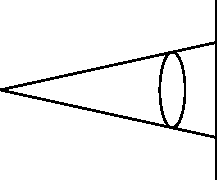
\includegraphics{epee_bocle/bocle_cone_proche}}
	\caption{Cônes de protections pour une bocle tenue loin et près.}
	\label{épée-bocle:fig:bocle-cone}
\end{figure}


\begin{exercice}[Défendre la main]

\D tend le bras droit devant lui et place sa main gauche près de sa main droite. 
\A essaie de toucher la main droite de \D qui ne peut se défendre qu'avec la main gauche.

Cet exercice travaille le fait de placer sa bocle du côté de l'épée adverse et de réagir vite pour l'intercepter.

Source : Arthur.

\end{exercice}


% fluidité
\begin{exercice}[Changements de garde]

Passer d'une garde à une autre en intercalant une frappe à chaque fois.
Chercher à être fluide.

\end{exercice}


\begin{exercice}[Couper la main]

\begin{enumerate}
	\item \A porte une attaque lente à \D, qui se défend simplement.
	\item Si une partie du corps de \A n'est pas protégée, alors \D amène son épée pour le mettre en évidence.
\end{enumerate}

\A peut enchaîner les frappes (en laissant le temps à \D de réagir pour mettre en évidence une éventuelle erreur).
Le but n'est pas d'aller vite mais de vérifier si la position est correcte.

Au début \D peut se concentrer uniquement sur la main d'arme de \A en faisant peu de mouvements, puis quand \A commence à avoir l'habitude \D peut chercher d'autres cibles et bouger légèrement.

\end{exercice}


\subsection{Gardes}


\begin{garde}[Crosse – \emph{Krucke}]
\index{krucke}
\index{garde!épée-bocle!krucke}

Dans la garde de la crosse (all. \emph{Krucke}, ang. \emph{crutch}), les mains sont placées face au visage, la pointe de l'épée vers le bas, la bocle couvrant la main d'arme.

\end{garde}

Cette garde est très hermétique et permet de dévier les estocs bas.


%%%%%%%%%%%%%%
\section{I.33}
%%%%%%%%%%%%%%


% type d'épée : Cinato : XVI, clubs allemands : XIV

% Royal Armouries, Tower Fechtbuch
Le traité MS I.33 (appelé aussi \emph{Walpurgis Fechtbuch} ou \emph{Liber de arte dimicatoria}) est le plus vieux manuel qui nous soit parvenu – il a été rédigé dans la décennie de 1320.
L'auteur serait un prêtre nommé Liutger.

La référence pour l'étude du I.33 est la traduction et le commentaire de Cinato et Suprenant~\cite{cinato:I33:2009}.
Kenner a écrit un manuel sur le sujet~\cite{kenner:I33:2014}.
Les images en couleur peuvent être trouvées sur le site de Wiktenauer~\cite{wiktenauer:I33}.


% TODO: custodia, contraria, liages supérieur/inférieur gauche/droit (inférieur = par en dessous)

\begin{definition}[Assiègement]
\index{assiègement}
\index{obsessio|see{assiègement}}
\index{contraria|see{assiègement}}

Un assiègement (lat. \emph{obsessio}~\cite{cinato:I33:2009}, \emph{contraria}~\cite{kenner:I33:2014}) est une position qui permet de briser une garde (lat. \emph{custodia}).

Il s'agit d'une position relativement hermétique et un assiègement adapté permet de se couvrir des attaques provenant de la garde adoptée par l'opposant.

\end{definition}

% liste des assiègement : krucke


\begin{definition}[Garde – \emph{Custodia}]
\index{garde!I.33}
\index{custodia|see{garde I.33}}

Une garde (lat. \emph{custodia}) est une position permettant de préparer une attaque.
Elle offre généralement une faible protection.

\end{definition}

% liste des gardes : 1 à 7

% TODO: déplacer en épée longue ?
\index{liage}
Il existe quatre liages possible : supérieur/inférieur et gauche/droite.
La personne qui lie est celle qui possède le centre et qui possède donc un avantage (plus ou moins important) sur l'autre.
Lorsque l'épée de celui qui lie est au-dessus on parle de liage supérieur, et de même si l'épée est en-dessous on parle de liage inférieur.
% cf Kenner

\begin{exercice}[Liages]

\begin{enumerate}
	\item \A fait un oberhau.
	\item \D vient prendre un liage.
	\item \A inverse le liage.
\end{enumerate}

L'oberhau est de hauteur variable pour encourager \D à varier les liages.
Le but n'est pas d'aller vite mais de sentir qui a le centre qui lie/est lié, de voir à quel point on est gêné et trouver le meilleur reliage.

\end{exercice}



%%%%%%%%%%%%%%%%%%%%
\section{Liegniczer}
%%%%%%%%%%%%%%%%%%%%


% TODO: add german words in techniques

Le traité de Liegniczer sur l'épée-bocle est très court et contient seulement six enchaînements.
On peut en trouver diverses transcriptions/traductions~\cite{ardamhe:liegniczer, farrell:liegnieczer, lindholm:ringeck_others:2006} ainsi que des interprétations~\cite{farrell:pedagogy_liegnieczer:2014, youtube:sala_armi:liegniczer, youtube:memag:liegniczer, lindholm:ringeck_others:2006, Myers:LiegniczerBuckler, knight:epee_bocle}.
Notre interprétation suit fortement~\cite{youtube:sala_armi:liegniczer, farrell:pedagogy_liegnieczer:2014}, ainsi que~\cite{youtube:memag:liegniczer}.

Le style développé par Liegniczer est très proche du système de Liechtenauer par le fait qu'il repose sur le concept de liage et de winden.
Il se rapproche aussi du I.33 par le fait que la bocle sert avant tout à couvrir la main d'arme, comme cela est indiqué dès le début de la première technique.
Keith Farrell a écrit un article sur la pédagogie de Liegniczer~\cite{farrell:pedagogy_liegnieczer:2014} afin de montrer que la structuration des six techniques présente bien un système cohérent et puissant.

Dans notre interprétation nous nous éloignons du livre de Lindholm, Svard and Clements~\cite{lindholm:ringeck_others:2006} qui ne nous semble pas correspondre tout à fait à l'esprit du système de Liegniczer : par exemple dans la technique 2, l'attaquant et les défenseurs séparent leurs deux mains.
% TODO: citer la page
De même l'interprétation de H.\ Knight~\cite[part I]{knight:epee_bocle} ne nous a pas convaincu, entre autres à cause des positions faibles qu'il adopte.

Dans chaque technique \A attaque tandis que \D est globalement passif : il semble que ce dernier ne soit pas initié à l'escrime et réagisse simplement avec des déflexions.
De même qu'en épée longue, \A va réagir d'une manière différente selon la réaction de \D, en apportant une réponse adaptée au mouvement de \D (ressenti).
% \emph{fühlen}
Ainsi qu'il a été expliqué plus haut, la bocle doit toujours protéger la main d'épée en se plaçant du même côté de l'épée de \D.
De même si \D ne prend pas soin de couvrir son bras alors \A doit frapper cette cible plus facile à atteindre.
Le seul moment où la bocle n'est pas utilisé pour couvrir la main est lorsque \A se trouve près de \D : dans ce cas la bocle est utilisée pour frapper et/ou contrôler les bras/mains de \D (entre autres lorsque l'on change d'axe ou que l'on vient chercher une cible basse).

L'idéal pour pratiquer ces techniques est de décomposer les techniques en séquences où \A doit réagir correctement selon ce que fait \D – d'abord en augmentant progressivement la longueur de l'enchaînement, puis en variant d'une fois à l'autre.


\begin{technique}[Liegniczer 1]
\label{épée-bocle:tech:liegniczer:1}

\A et \D démarrent dans la custodia 2 (épaule droite).

\begin{enumerate}
	\item \A lance un oberhau sur l'épaule droite de \D, en avançant la jambe droite.
	
	\item \D pare avec un oberhau, en avançant la jambe droite, et prend le liage.
	
	\item \alt{Si \D est faible, \A estoque.}
		Si \D est relativement fort au liage, \A exécute un winden en levant les mains en bœuf (en supination ou en pronation).
	
	\item \alt{Si \D ne réagit pas, \A estoque.}
		Si \D pousse la lame vers l'extérieur alors \A quitte le liage et vient frapper \D de l'autre côté en passant sous la lame (\emph{schnappen}),
		tout en frappant les mains de \D avec la bocle pour éloigner la menace.
\end{enumerate}

Au temps 3) le plus simple est de lever directement la main en supination ; cette position est relativement faible si l'on n'utilise pas le pouce en appui comme expliqué dans l'introduction de ce chapitre.
Le \emph{schnappen} au temps 4) sera d'autant plus efficace que \D écarte fort la lame – à l'extrême si \D écarte fort dès le temps 2) alors il n'y a pas de winden.

Pour illustrer nos explications générales, \A n'a pas besoin d'exécuter l'ensemble de la technique si \D fait une erreur.
Par exemple si \D est faible au temps 2) alors \A peut estoquer directement.

Au temps 2) les rôles sont symétriques et \D peut prendre l'initiative, auquel cas les rôles s'inversent.
De ce point de vue une autre manière d'interpréter l'enchaînement est que \D attaque \A qui prend le liage avec un oberhau, et ensuite enchaîne.

\end{technique}


\begin{figure}[htp]
	\centering
	\includegraphics{diagrammes/epee_bocle/liegniczer_1}
	\caption{Diagramme pour la technique 1 de Liegniczer.
	Nous n'indiquons pas le cas où \D ne réagit pas au premier oberhau.}
	\label{épée-bocle:fig:liegniczer:diagramme-1}
\end{figure}



\begin{technique}[Liegniczer 2]
\label{épée-bocle:tech:liegniczer:2}

\A démarre dans la custodia 5 (queue), \D dans la custodia 2 (épaule droite).

\begin{enumerate}
	\item \A lance un unterhau en avançant la jambe droite.
	
	\item \D prend le liage avec un oberhau en avançant la jambe droite.
	
	\item \alt{Si \D est faible, \A estoque.}
		Si \D est fort \A exécute un winden en levant les mains.
	
	\item \alt{Si \D ne réagit pas, \A estoque.}
		Si \D repousse la lame, \A exécute un duplieren tout en se décalant sur la gauche.
		La bocle permet de coincer l'épée de \D.
	
	\item \D se protège du coup et \A vient frapper les jambes du vrai tranchant (dans l'intérieur de \D).
\end{enumerate}

Il est possible d'inverser les temps 1) et 2) si l'on voit l'unterhau de \A comme un liage (inférieur).

\D se trouve naturellement jambe droite devant et il s'agit de la cible principale, alors que le traité indique que \A vise la jambe gauche : une interprétation est que \D peut toujours reculer la jambe droite, mais pas la gauche et si l'on vise cette dernière (ce qui est possible comme le coup est à l'intérieur) alors on est sûr de toucher quelque chose.

\end{technique}

% talhoffer : Myers:LiegniczerBuckler, knight:epee_bocle


\begin{technique}[Liegniczer 3]
\label{épée-bocle:tech:liegniczer:3}
% \index{coup!allemand!wechselhau}

\A et \D démarrent dans la custodia 2 (épaule droite).

\begin{enumerate}
	\item \A lance un oberhau en avançant la jambe droite.
	
	\item Quand \D se protège, \A laisse tomber la pointe de son épée sous celle de \D et la relève ensuite en battant fortement l'épée de \D avec le faux tranchant (coup changeant, wechselhau).
		\A se sert de l'élan pour frapper (du vrai tranchant) la tête de \D du côté droit en avançant la jambe gauche.
	% mouvement de hanches pour le balayage : permet d'éviter l'attaque ?
	
	\item \D se protège et \A exécute un winden en tournant la main en supination.
	
	\item \alt{Si \D ne fait rien, \A estoque.}
		\D dévie l'estoc et \A vient frapper la jambe droite du vrai tranchant.
		La bocle écarte les mains de \D.
\end{enumerate}

Au temps 2) le balayage est exécuté avec le faux tranchant car cela est plus rapide qu'avec le vrai, qui nécessiterait plusieurs rotations du poignet.
Il est aussi important de passer la bocle du côté droit du bras d'arme lors de la frappe, autant pour protéger le bras que pour laisser ouverte la ligne basse d'attaque.

La position en 3) n'est pas très forte : à notre avis l'idée est de surprendre en changeant la ligne d'attaque (technique~\ref{struct:tech:changement-ligne}).

Dans ce contexte la première attaque est une feinte.
Une autre interprétation est possible si \A commence dans la garde du fou : dans ce cas la déflexion en 2) est utilisée contre un oberhau de \D (pour une garde à gauche le balayage se fera naturellement avec le vrai tranchant).

\end{technique}


\begin{technique}[Liegniczer 4]
\label{épée-bocle:tech:liegniczer:4}
% \index{coup!allemand!mittelhau}

\A et \D démarrent dans la custodia 2 (épaule droite).

\begin{enumerate}
	\item \A lance un mittelhau (avec le vrai tranchant) à droite en avançant la jambe droite.
	
	\item \D se protège et \A frappe de l'autre côté avec un second mittelhau (vrai tranchant) en avançant la jambe gauche.
	
	\item \D se protège et \A lance un coup crânien (vrai tranchant) en avançant la jambe droite.
	
	\item \D se protège et \A fait glisser l'épée le long de la bocle de \D pour estoquer le ventre.
		\A garde sa bocle haute pour empêcher \D de baisser ses mains et pour protéger sa tête.
\end{enumerate}

L'idée de l'enchaînement est d'exécuter une série rapide de plusieurs coups qui vise à faire progressivement monter les défenses de \D afin d'attaquer bas à la fin.
Cela marche d'autant mieux si l'on a pu faire entrer \D dans un schéma, par exemple en lançant plusieurs mittelhau à la suite (par exemple avec un enchaînement droit-bas puis gauche-haut).

Les temps 1) et 2) constituent un double zwerchau, où la différence par rapport à l'épée longue est que la première frappe est faite avec le vrai tranchant.
Il est en effet un peu plus difficile de tourner la main sur la garde pour une épée une main puisque la main gauche n'est pas là pour stabiliser, et en gardant le pouce en appui sur les quillons il n'est pas possible de frapper avec le faux tranchant au temps 2) et 3).

Au temps 4) \A ne doit pas ramener son épée en arrière pour estoquer car il perdrait le centre (et du temps).

\end{technique}


\begin{technique}[Liegniczer 4 (variante)]
\label{épée-bocle:tech:liegniczer:4v}

\A et \D démarrent dans la custodia 2 (épaule droite).

\begin{enumerate}
	\item \A lance un mittelhau (avec le faux tranchant) à droite en avançant la jambe droite.
	
	\item \D se protège et \A frappe de l'autre côté avec un second mittelhau (vrai tranchant) en avançant la jambe gauche.
	
	\item \D se protège et \A lance un coup crânien (faux tranchant) en avançant la jambe droite.
	
	\item \D se protège et \A fait glisser l'épée le long de la bocle de \D pour estoquer le ventre.
		\A garde sa bocle haute pour empêcher \D de baisser ses mains et pour protéger sa tête.
\end{enumerate}

La différence avec la variante précédente est que deux des attaques – temps 1) et 3) – se font avec le faux tranchant, et ainsi la première attaque ressemble plus au zwerchau allemand que dans la première version.
Cet enchaînement est possible à condition que le pouce soit placé au niveau de la croix quillons/poignée, comme en épée longue, et que l'on conserve cette position tout le long.

Avec cette tenue la frappe en 3) avec le faux tranchant est très naturelle et plus rapide que si l'on devait ramener le vrai tranchant, et l'on dispose aussi d'un plus grand angle pour estoquer derrière la bocle (du fait de la position du poignet).

% Léo
\end{technique}


Une autre variante est proposée dans~\cite{youtube:sala_armi:liegniczer} : les mittelhaus sont respectivement portés à gauche et à droite.
Nous pensons que cet ordre est moins intéressant car il est quasiment certain qu le coup crânien tombera sur le bouclier ; mais cela reste une variation intéressante qui peut surprendre l'adversaire.


\begin{technique}[Liegniczer 5]
\label{épée-bocle:tech:liegniczer:5}

\A et \D démarrent dans la custodia 2 (épaule droite).

\begin{enumerate}
	\item \A lance un oberhau à droite en avançant la jambe droite, et tout en frappant tourne son poignet de 90° (sens direct) pour amener la pointe vers le bas, derrière le bouclier de \D (coup plongeant, sturtzhau).
	
	\item \alt{Si \D ne fait rien, \A estoque.}
		\D dévie l'estoc et \A fait contourne la bocle avec sa pointe pour venir estoquer le ventre : soit en descendant (rotation du poignet), soit en montant (rotation de l'épaule).
	
	\item \alt{Si \D ne fait rien, \A estoque.}
		\D dévie l'estoc (par exemple en passant en \emph{Krucke}) et \A exécute un winden en tournant la main en supination.
	
	\item \alt{Si \D ne fait rien, \A estoque.}
		\D dévie l'estoc vers sa droite et \A vient frapper la jambe droite du vrai tranchant.
		La bocle écarte les mains de \D.
\end{enumerate}

Au temps 1) l'oberhau est une feinte (mais si \D ne bouge pas alors il n'y a pas besoin de l'exécuter).
La fin de la technique est très similaire à celle de la séquence~3 (technique~\ref{épée-bocle:tech:liegniczer:3}).

Comme indiqué en 2) le contournement de la bocle peut se faire de deux manières.
Plusieurs interprétations favorisent un estoc descendant (en rapport avec la variante suivante), mais l'estoc montant semble favorisé dans la traduction de l'\textsc{Ardamhe}~\cite{ardamhe:liegniczer} : "monte la pointe par dessous".

Au temps 3) nous avons noté qu'une bonne défense pour \D est le \emph{Krucke}.
Elle est particulièrement adaptée si l'estoc est bas, mais elle ne correspond pas à une défense "naïve".
En Krucke \D peut sembler être protégé aux jambes : en fait lorsqu'il dévie l'estoc il commence à s'ouvrir, et la bocle permet d'écarter encore plus sa lame.

\end{technique}


\begin{technique}[Liegniczer 5 (variante)]
\label{épée-bocle:tech:liegniczer:5v}

\A et \D démarrent dans la custodia 2 (épaule droite).

\begin{enumerate}
	\item \A lance un oberhau à droite en avançant la jambe droite, et tout en frappant tourne son poignet de 90° (sens direct) pour amener la pointe vers le bas, derrière le bouclier de \D (coup plongeant, sturtzhau).
	
	\item Avant que \D ne dévie la pointe, \A contourne la bocle de \D grâce à une rotation du poignet, afin d'estoquer le côté droit de \D.
	
	\item \alt{Si \D ne fait rien, \A estoque.}
		\D dévie l'estoc et \A exécute un winden en tournant la main en supination.
	
	\item \alt{Si \D ne fait rien, \A estoque.}
		\D dévie l'estoc vers sa droite et \A vient frapper la jambe droite du vrai tranchant.
		La bocle écarte les mains de \D.
\end{enumerate}

Dans cette variante \A exécute deux feintes : d'abord en inversant la direction de la lame, puis en contournant la bocle.
Dans ce cas-là l'estoc au temps 2) est plus haut et \D devra utiliser une garde haute pour le dévier.

\end{technique}

\begin{figure}[htp]
	\centering
	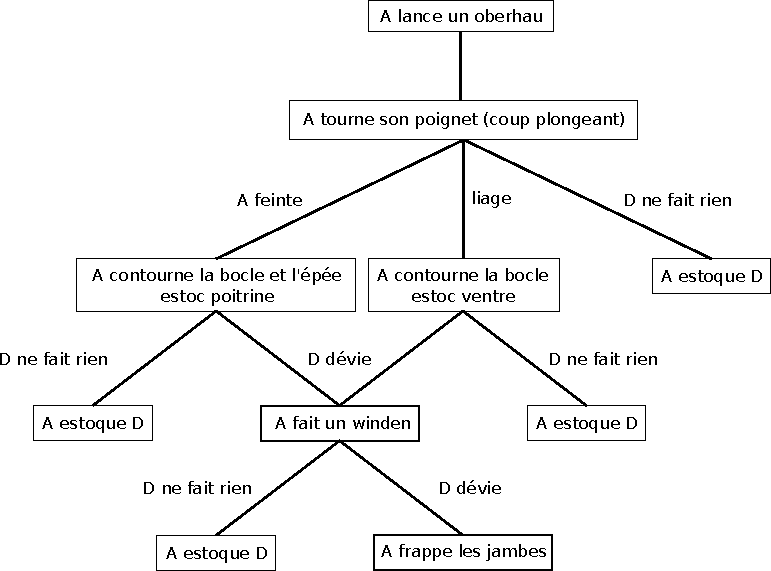
\includegraphics{diagrammes/epee_bocle/liegniczer_5}
	\caption{Diagramme pour la technique 5 de Liegniczer.}
	\label{épée-bocle:fig:liegniczer:diagramme-5}
\end{figure}


\begin{technique}[Liegniczer 6]

\A démarre dans une garde basse, \D dans la custodia 2 (épaule droite).

\begin{enumerate}
	\item \D lance un oberhau à droite en avançant la jambe droite.
	
	\item \A passe en demi-épée et fait une parade franche.
	
	\item \A lâche sa main droite et attrape la bocle de \D.
	
	\item \A arrache la bocle de \D.
	
	\item \A utilise la bocle pour frapper \D au visage.
\end{enumerate}

La meilleure manière pour retirer la bocle est de l'attraper par en-dessous (avec la paume tournée vers la droite) et de tourner dans le sens horaire~\footnotemark{}.
\footnotetext{Attention en pratiquant avec un partenaire : s'il a des gants épais ils peuvent rester coincés sous la poignée et la torsion peut être douloureuse.}

\A peut directement démarrer en demi-épée mais son intention peut alors être devinée plus facilement, sauf si la main est cachée par la bocle – par exemple grâce à la custodia 1 (sous le bras) ou si l'échange commence hors distance et \A adopte une position reposante.

À partir du moment où \A lâche sa poignée il doit la garder hors d'atteinte de \D.

\end{technique}

